Wenn du jetzt das Minecraft-Profil “forge” startest, solltest du eine neues Mainmenu sehen:

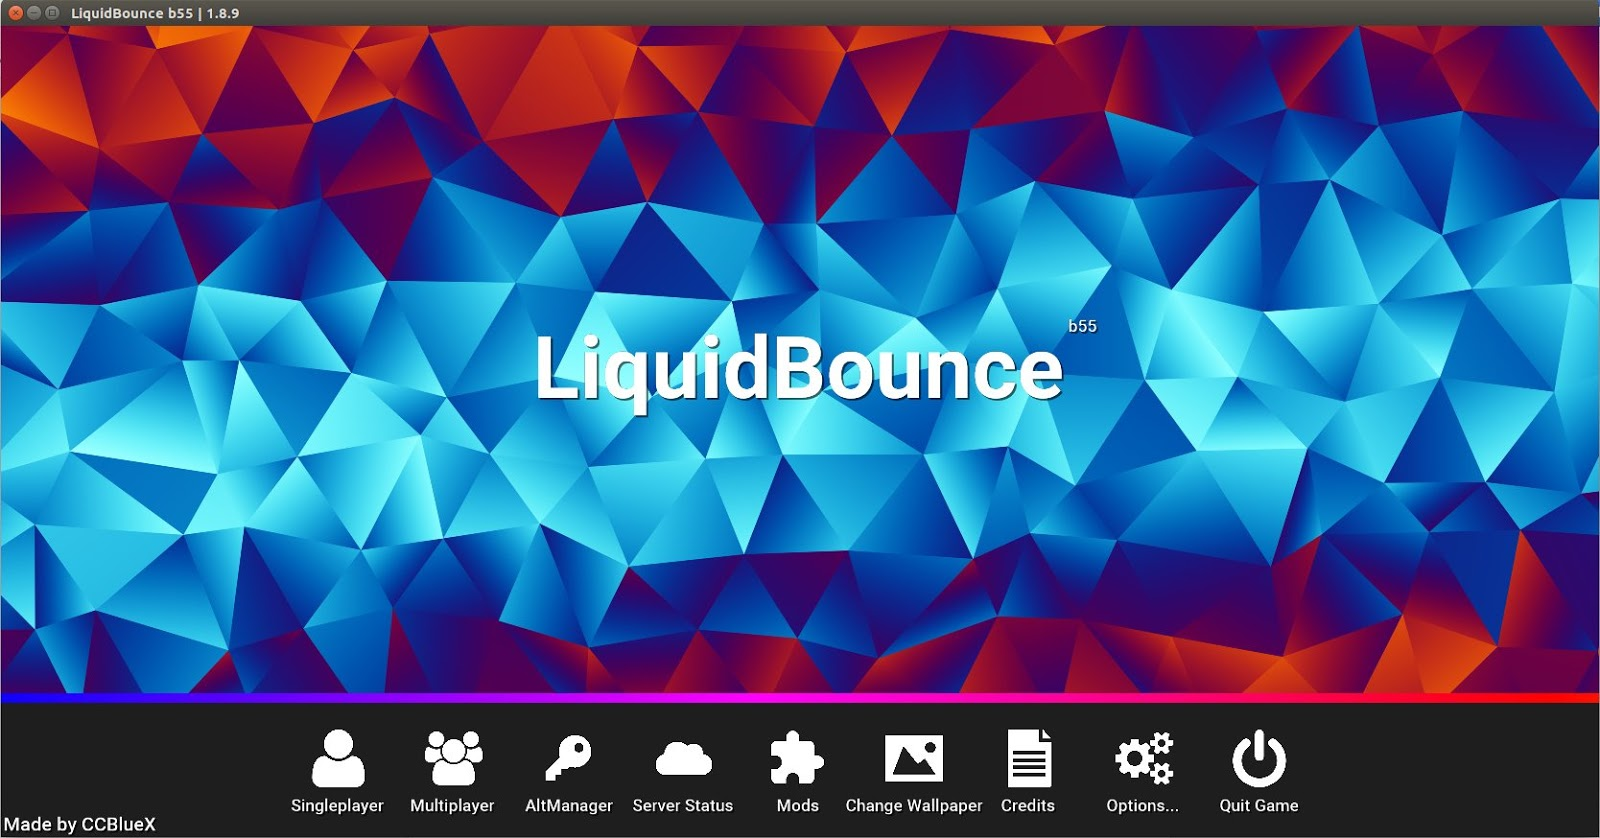
\includegraphics[width=0.7\textwidth, center]{TeX_files/pics/erster_start_1_8.jpg}

Für die Minecraft-Version 1.12.2 sieht das Mainmenu so aus:

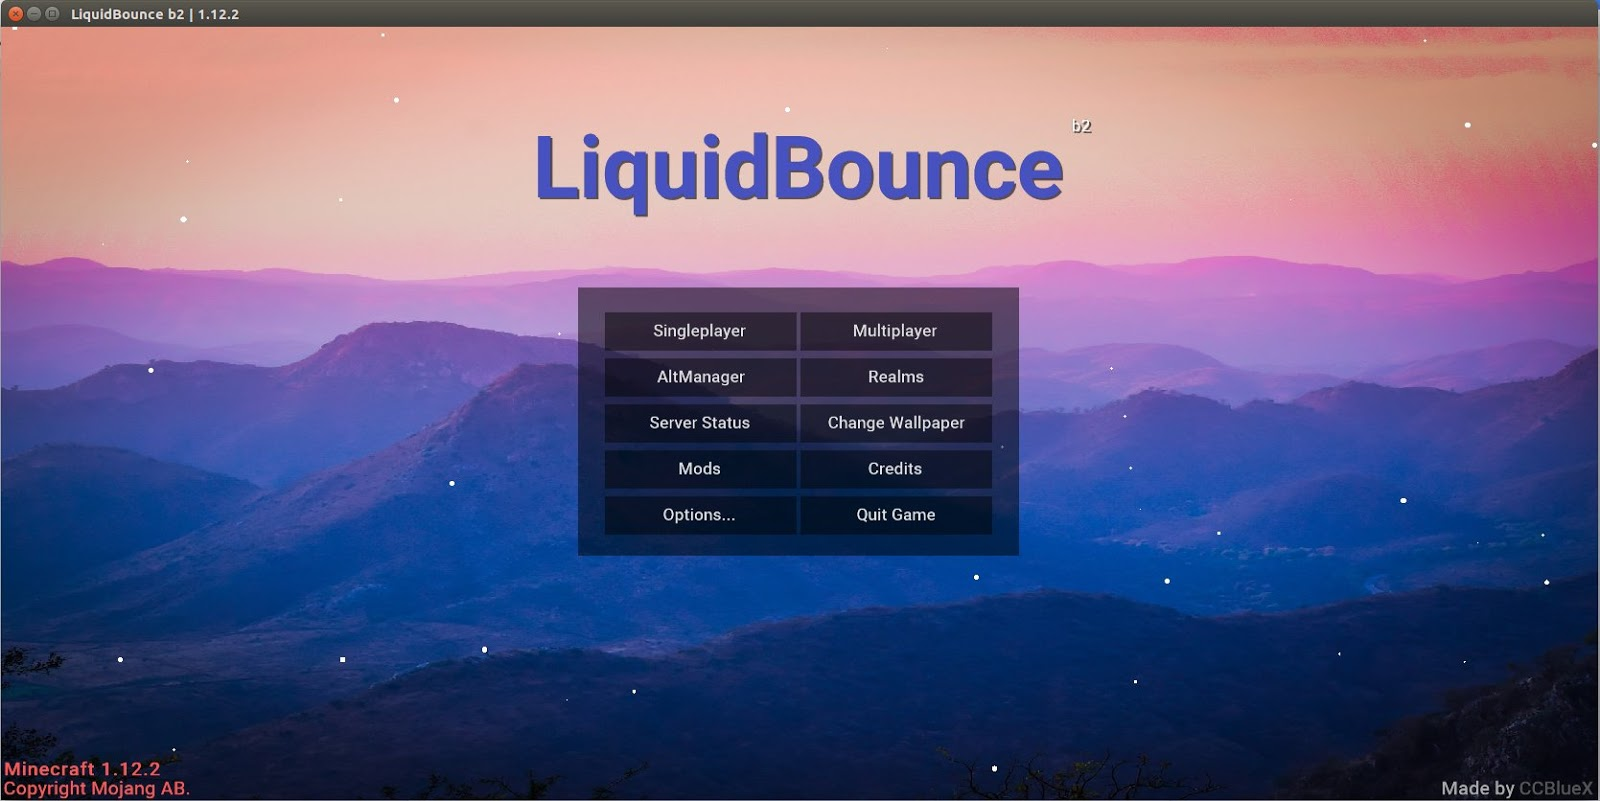
\includegraphics[width=0.7\textwidth, center]{TeX_files/pics/erster_start_1_12.jpg}

Vielleicht kommt noch ein Hinweis, der in wenigen Worten die Handhabung erklärt, aber den kann man auch schnell wegklicken.

Für den Anfang solltest du in eine Singleplayer-Welt gehen und dort alles ausprobieren. Der wichtigste Befehl am Anfang ist: \texttt{.bind clickgui LCONTROL} (Befehle beginnen immer mit einem Punkt und werden ganz normal in den Chat eingegeben, also insbesondere ohne den führenden \texttt{/})

Wenn du jetzt die linke Strg-Taste drückst, öffnet sich das ClickGUI

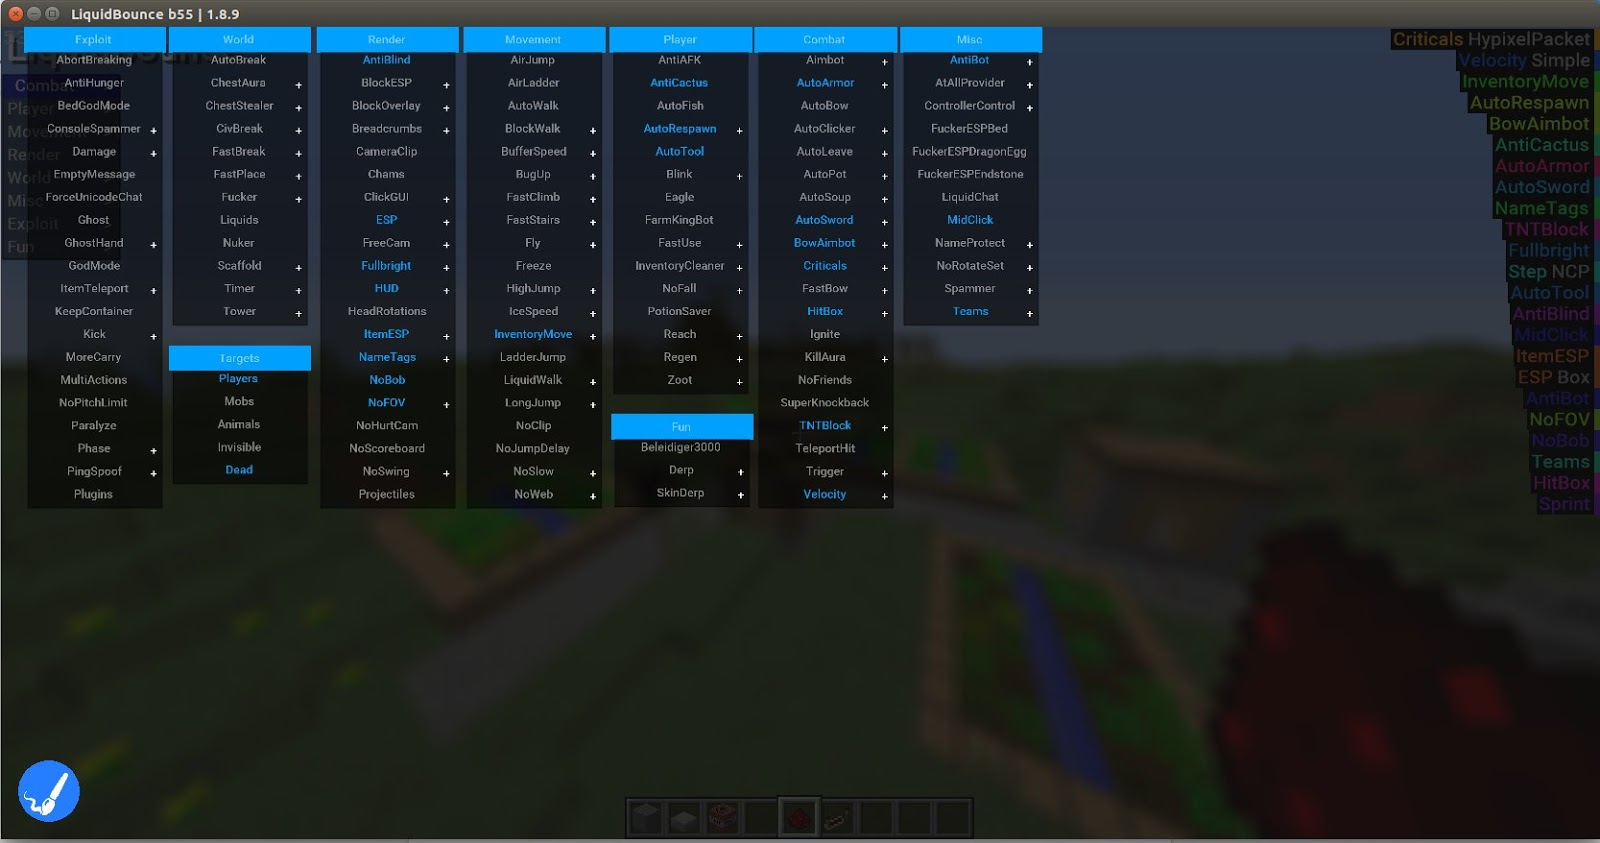
\includegraphics[width=0.7\textwidth, center]{TeX_files/pics/clickgui.jpg}

Die blauen Reiter lassen sich mit Rechtsklick öffnen bzw. schließen und mit gedrückter linker Maustaste bewegen.

Mit dem blauen Pinsel links unten kannst du dein HUD - also zum Beispiel die Liste mit den Hacks, die Anzeige der gerade aktiven Effekte, usw. - verändern. Aber meiner Meinung nach muss man da nichts ändern.

Module (also die Hacks) kann man mit einem einfachen Linksklick aktivieren bzw. auch deaktivieren. Einige Module haben auch weitere Einstellungen, das erkennt man an dem $+$ rechts neben dem Hack. Diese Einstellungen lassen sich mit einem Rechtsklick öffnen und auch wieder schließen. Achtung: In der Regel öffnen sich diese Einstellungen unter den Listen der Reiter, also musst du erst die überdeckende Liste einfahren (Rechtsklick auf den Reiter) und die Einstellungen zu sehen und zu bearbeiten.
